\section{Theory} \label{sec:theory}
Mass-spectrometers are used to measure the amounts of different compounds in a gas. The gas is first ionized and then the different compounds are split up according to their charge-to-mass ratio. In this experiment we used a quadrupole-mass-spectrometer. A schematic view is shown in figure \ref{fig:schem}.
\begin{figure}[h!]
\centering
    \begin{circuitikz}[ scale=0.9,
                 	>=stealth',
                 	pos=.8,
                 	longL/.style = {cute choke, inductors/scale=0.75,
       inductors/width=1.6, inductors/coils=9}]
    \draw[] (-3,0) to [short] (0,0)
                 to [L] (0,-1)
                 to [short] (-1,-1)
                 to [short] (-1,-3)
                 to [short] (-1.5,-3);
    \draw[] (-3,0) to [short] (-3,-3)
                 to [short] (-2.5,-3)
                 to [battery1, l=$U_h$] (-1.5,-3);
                 
    \draw[] (-1,-3) to [battery1, l=$U_a$] (10,-3)
                      to [ammeter] (10,-0.5)
                      to [short] (9,-0.5);
                      
    \draw[] (9,-1) to (9,0);
    
    \draw[] (5,0.75) to [longL] (8,0.75)
                     to [short] (8,2.5)
                     to [battery1, l=$U$] (7,2.5)
                     to [sV, l=$V$] (5,2.5)
                     to [short] (5,0.75);
    
    \draw[] (5,0.5) rectangle (8,0.25);
    \draw[] (5,-1.25) rectangle (8,-1.5);
    \draw[dotted] (5,0.25) to (5,-1.25);
    \draw[dotted] (8,0.25) to (8,-1.25);
    
    \node at (1.25, 0.3) {e$^-$};
                      
    \draw[->, thick] (0.5,-0.2) to (2,-0.2);
    \draw[->, thick] (0.5,-0.5) to (2,-0.5);
    \draw[->, thick] (0.5,-0.8) to (2,-0.8);
    
    \node at (2.7,3.5) {probe};
    \node at (0,3.5) {filament};
    \node at (6.5,3.5) {quadrupole field};
    \node at (10,3.5) {detector};
    
    \node at (9,0.5) {A};
    \node at (0,0.5) {K};

    
    \filldraw[red] (2.4,-0.3) circle (0.2);
    \filldraw[red] (2.5,-0.8) circle (0.2);
    \filldraw[red] (2.7,0.1) circle (0.2);
    \filldraw[blue] (2.6,0.7) circle (0.2);
    \filldraw[blue] (2.3,-1.3) circle (0.2);

    \filldraw[blue] (3.2,-0.75) circle (0.2);
    \draw[blue, very thick, ->] (3.5,-0.75) to (5,-0.75) to [bend left = 30] (6,-1.25);

    \filldraw[red] (3.2,-0.2) circle (0.2);
    \draw[red, very thick,->] (3.5,-0.2) to (5,-0.2) cos (5.5,-0.4) sin (6,-0.6)
                                      cos (6.5,-0.4) sin (7,-0.2) cos (7.5,-0.4)
                                      sin (8,-0.6) to (9,-0.6);
                                      
    \draw[ultra thick, ->] (11,-1.75) to (12,-1.75);
    \draw[rounded corners] (12.25, -2.5) rectangle (13.75, -1) {};
    \node at (13,-1.75) {ADC};

    \end{circuitikz}
    \caption{Schematic view of a quadrupole-mass-spectrometer. The probe consists of red and blue elements. The setup is configured such that the red ions will follow a resonating path and arrive at the detector. The blue ions will follow a non-resonating path and are lost in the walls. When an ion hits the detector (anode A) a current will flow and is measurable with the Ammeter.}
    \label{fig:schem}
\end{figure}

\subsection{Working principle}
    The gaseous probe is first ionized. This is done by electrons that are detached from a glowing filament and accelerated by an electric field. They then hit the compounds of the probe.  The newly generated ions are then also accelerated by the electric field and guided through a electrodynamic quadrupole field. The three components of the equations of motion 
    \begin{equation}
        \begin{aligned}
            \ddot x + \left(\frac{q}{mr_0^2}\right)\Phi_0\cdot x= 0 \\
            \ddot y - \left(\frac{q}{mr_0^2}\right)\Phi_0\cdot y= 0 \\
            \ddot z = 0 
            \label{eq:quadstatic}
        \end{aligned}
    \end{equation}
    are given in the manual \cite{manual}.
    We see that the ions will move uniformly in the $z$ direction (along the electric field) but will follow a sinusoidal path in the $xz$-plane and an exponential path in the $yz$-plane which will direct them into the walls. To mitigate this problem we will also apply an alternating voltage, this will give us the following equations of motion: \eqref{eq:quadalt}
    \begin{equation}
        \begin{aligned}
            \ddot x + \left(\frac{q}{mr_0^2}\right)(U-V\cos(\omega t))\cdot x= 0 \\
            \ddot y - \left(\frac{q}{mr_0^2}\right)(U-V\cos(\omega t))\cdot y= 0 \\
            \ddot z = 0 
            \label{eq:quadalt}
        \end{aligned}
    \end{equation}
    where $U$ is the DC-offset and $V$ the amplitude of the alternating voltage.
    The $y$-axis will act as a low-pass and the $x$-axis as a high pass, together they form a bandpass filter that only lets certain charge-to-mass ratios pass through to the detector. By adjusting the DC-offset and the alternating voltage amplitude we are able to create a stable path, that lets just one component pass through (see figure \ref{fig:schem}). The parameters $a$ and $q$ 
    \begin{equation}
        \begin{aligned}
            a = \frac{4eU}{m\omega^2r_0^2} \\
            q = \frac{2eV}{m\omega^2r_0^2}
            \label{eq:params}
        \end{aligned}
    \end{equation}
    are defined in the manual \cite{manual}.
    The parameter $v=a/q=2U/V$ is independent of the charge-to-mass ratio and is describes the slope in the parameter space as shown in figure \ref{fig:paramspace}.
    \begin{figure}[h!]
    \centering
    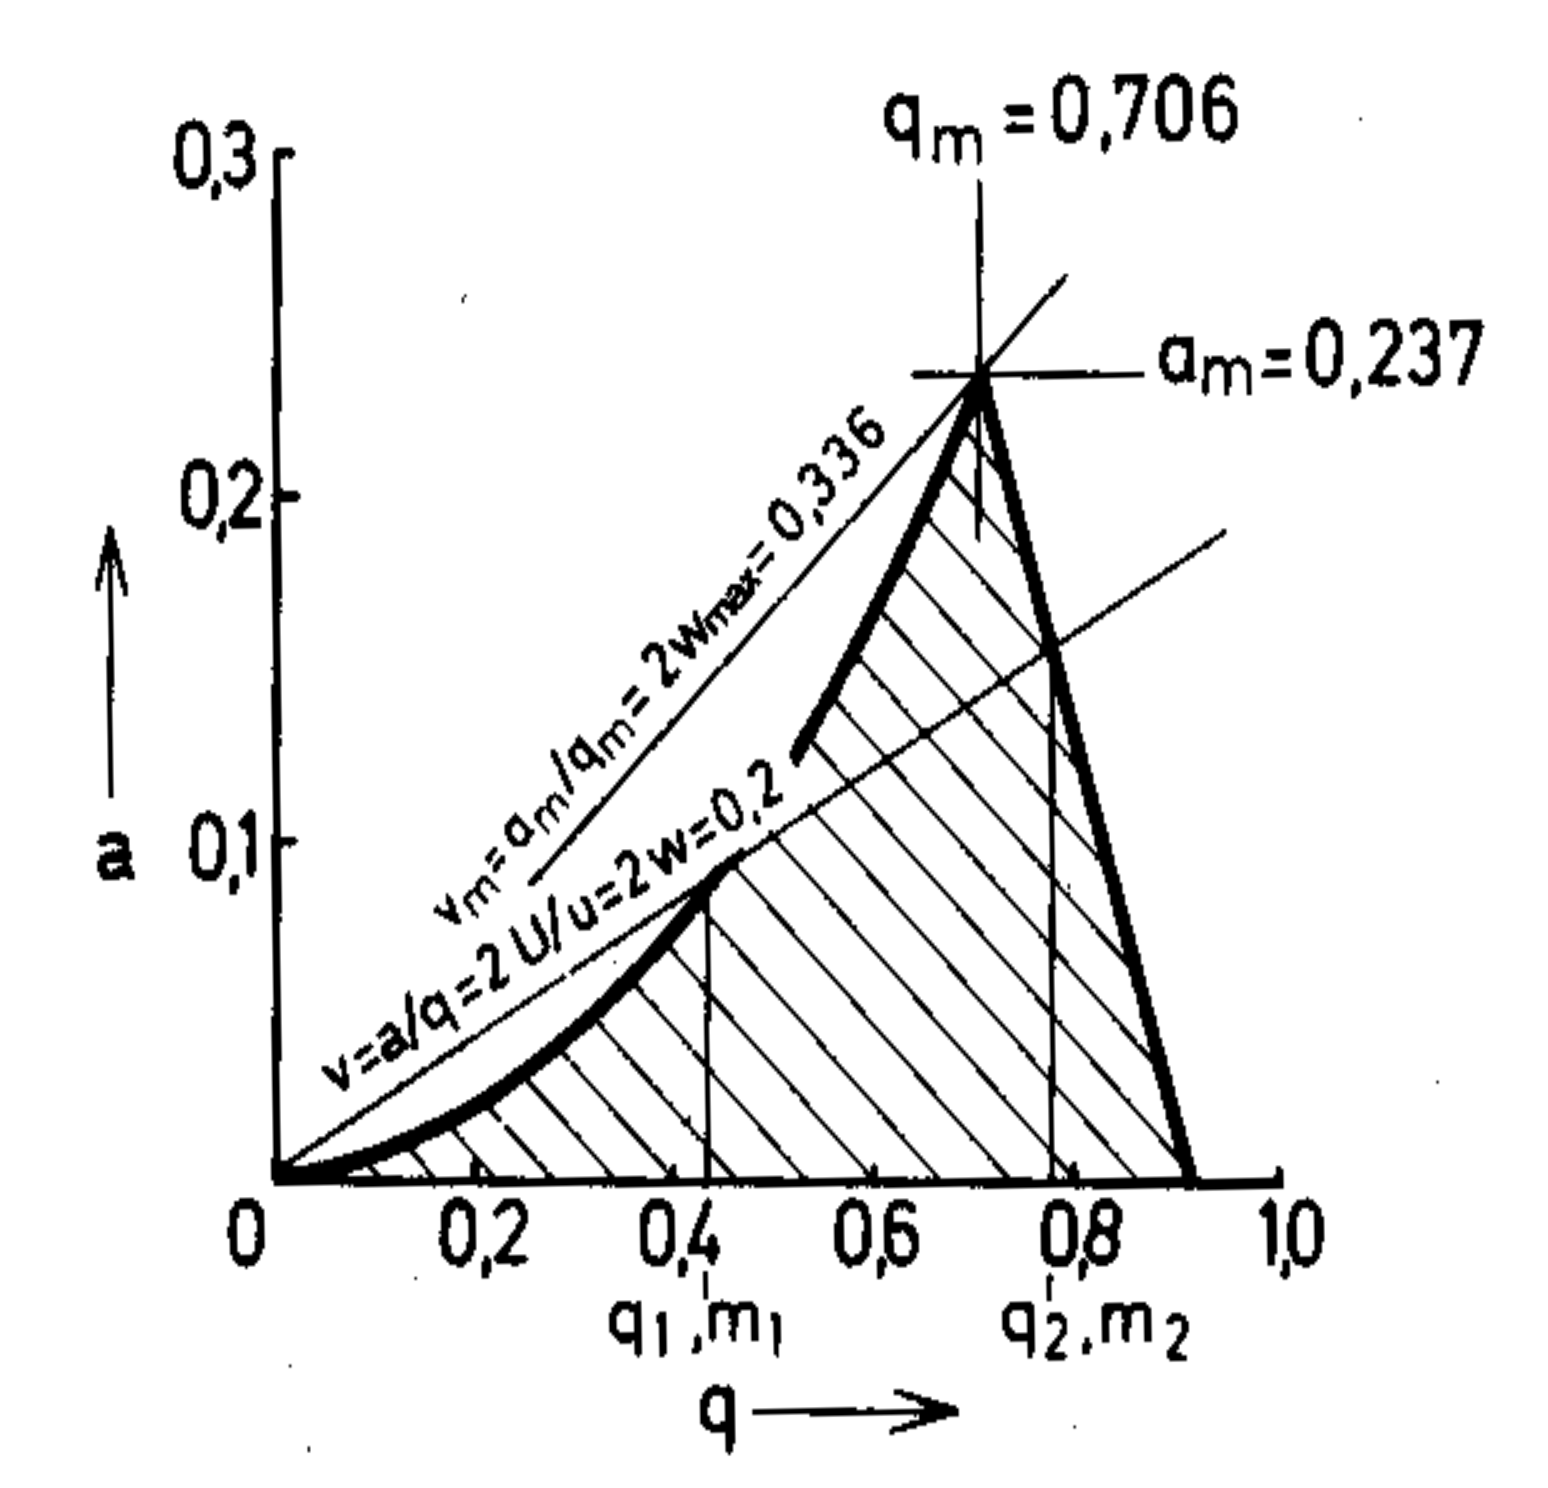
\includegraphics[width=0.4\textwidth]{Report/pictures/paramspace.png}
    \caption{The parameter space described by $a$ and $q$. \cite{manual}}
    \label{fig:paramspace}
    \end{figure}
    
    For measurements, $a$ and $q$ are changed so that we always work along this slope.  How this slope is chosen strongly influences the result. If the slope is too small, the resolution of the mass spectrometer is reduced because too many ions pass through. If it is too large, too few ions reach the detector, which reduces the sensitivity. 
    
    % TODO
    % write something about resolution and delta m
    
    \pagebreak
    \subsection{Detectors}
    \subsubsection{{\scshape Faraday} Detector}
    
    \begin{figure}[h!]
    \centering
        \begin{circuitikz}[ scale=0.9,
                     	>=stealth',
                     	pos=.8,
                     	longL/.style = {cute choke, inductors/scale=0.75,
           inductors/width=1.6, inductors/coils=9}]
        
        \draw[very thick, red, ->] (0,-1) -- (5,-1);
        \draw (2,0) to (5,0) to (5,-3) to (2,-3);
        \draw (5,-1.5) to[short] (7,-1.5) to[ammeter] (7,-4) node[ground] {};
        \end{circuitikz}
        \caption{Schematic view of a {\scshape Farraday}-Detector.}
        \label{fig:Farraday}
    \end{figure}
    
    A {\scshape Faraday} Detector is a simple device as shown in figure \ref{fig:Farraday} which consists of a conductor surface connected to an ampere meter. If an Ion hits the surface, the Ion is neutralised and the conductor charged, this leads to a current flowing to ground, which is proportional to the number of Ion hits. Since there is no active amplification, this detector is not as sensitive as the SEM. It can operate at pressures of $10^{-11}$ Torr \cite{manual}.
    
    \subsubsection{Secondary Electron Multiplier (SEM)}
    
    \begin{figure}[h!]
    \centering
        \begin{circuitikz}[ scale=0.9,
                     	>=stealth',
                     	pos=.8,
                     	longL/.style = {cute choke, inductors/scale=0.75,
           inductors/width=1.6, inductors/coils=9}]
        
        \node at (3.5,1) {Continuous Dynode};
        \draw (7,-1) to[ammeter] (9,-1) node[ground] {};
        \draw (0,0) to (0,0.5) node[anchor=south] {V+};
        \draw[thick] (0,0.5) circle (0.1);
        \filldraw[thick] (0,0.5) circle (0.03);

        \draw[thick, red, ->] (-2,-2) to (0.5,0.2);
        \draw[thick, red, ->] (0.5,0.2) to (1.5,-0.8);
        \draw[thick, red, ->] (0.5,0.2) to (1.4,-0.85);
        \draw[thick, red, ->] (0.5,0.2) to (1.6,-0.75);
        \draw[thick, red, ->] (1.5,-0.8) to (3, 0.6);
        \draw[thick, red, ->] (1.5,-0.8) to (3.1, 0.6);
        \draw[thick, red, ->] (1.4,-0.85) to (2.9, 0.6);
        \draw[thick, red, ->] (1.4,-0.85) to (2.8, 0.6);
        \draw[thick, red, ->] (1.6,-0.75) to (3.2, 0.6);
        \draw[thick, red, ->] (1.6,-0.75) to (3.3, 0.6);
        \draw[thick, red, ->] (3, 0.6)  to  (5,-0.2);
        \draw[thick, red, ->] (2.9, 0.6) to (5,-0.05);
        \draw[thick, red, ->] (2.8, 0.6) to (5,0.1);
        \draw[thick, red, ->] (3.2, 0.6) to (5,0);
        \draw[thick, red, ->] (3.3, 0.6) to (5,-0.1);
        
        \draw[ultra thick] (0,0) to[bend left = 30] (7,-1);
        \draw[ultra thick] (0,-2) to[bend left = 40] (7,-1);
        
        
        
        \end{circuitikz}
        \begin{circuitikz}[ scale=0.9,
                     	>=stealth',
                     	pos=.8,
                     	longL/.style = {cute choke, inductors/scale=0.75,
           inductors/width=1.6, inductors/coils=9}]
        

        \draw[thick, red, ->] (-2, -6) to (0.3,-3.8);

        \node at (4.5,-2.5) {Discrete Dynode};
        
        \draw[thick, red, ->] (0.3,-3.8) to (1.35,-6) to (2.35,-3.8);
        \draw[thick, red, ->] (0.3,-3.8) to (1.25,-6) to (2.25,-3.8);

        \foreach \i in {0,2,...,6}{
            \draw (\i+0.3,-3.8) to (\i+0.3,-3.6) to (\i+0.5,-3.6);
            \draw (\i+0.5,-3.7) rectangle (\i+1,-3.5);
            \draw (\i+1.5,-3.7) rectangle (\i+2,-3.5);
            \draw (\i+1,-3.6) to (\i+1.5,-3.6);
            \draw (\i+2,-3.6) to (\i+2.3,-3.6);
            \draw[dashed] (\i+1.25,-3.6) to (\i+1.25,-6);
            
            \draw[thick, red, ->] (\i+0.3,-3.8) to (\i+1.3,-6) to (\i+2.3,-3.8);
            \foreach \j in {0,...,\i}{
                \draw[thick, red, ->] (\i+\j/30+0.3,-3.8) to (\i+\j/30+1.3,-6) to (\i+\j/30+2.3,-3.8);
                 \draw[thick, red, ->] (\i-\j/30+0.3,-3.8) to (\i-\j/30+1.3,-6) to (\i-\j/30+2.3,-3.8);
            }
            
            \draw[ultra thick] (\i,-4) -- (\i+0.1,-3.8) -- (\i+0.5,-3.8) -- (\i+0.6,-4);
            \draw[ultra thick] (\i+1,-5.8) -- (\i+1.1,-6) -- (\i+1.5,-6) -- (\i+1.6,-5.8);

        }
        
        \draw (0.3,-3.6) to (0.3,-3) node[anchor=south] {V+};
        \draw[thick] (0.3,-3) circle (0.1);
        \filldraw[thick] (0.3,-3) circle (0.03);
        \draw (8.3,-3.6) to[short] (9,-3.6) to[ammeter] (11,-3.6) node[ground] {};

        
        \end{circuitikz}
        \caption{Schematic view of SEM-Detectors.}
        \label{fig:SEM}
    \end{figure}
    
    As shown in figure \ref{fig:SEM} an SEM can be in a continuous Dynode setup or in a discrete Dynode setup. The SEM can amplify an incident Ion. The Ion hits a Dynode which emits secondary electrons, which are accelerated in the electric field generated by the voltage V+. This leads to electron avalanches. The induced current can be easily measured. Due to the amplification, this detector can operate at pressures of $10^{-14}$ Torr \cite{manual}. However the noise is also larger because ambient radiation can also cause electron avalanches that are then measured. The surfaces suffer from more wear because of the continuous electron bombardment.